\documentclass[12pt]{article}
\usepackage[danish]{babel}
\usepackage{amsfonts, amssymb, mathtools, amsthm, amsmath}
\usepackage{graphicx, pgfplots}
\usepackage{url}
\usepackage[dvipsnames]{xcolor}
\usepackage{sagetex}
\usepackage{lastpage}

%loaded last
\usepackage[hidelinks]{hyperref}

\usepackage{siunitx}
  \sisetup{exponent-product = \cdot,
    output-decimal-marker = {,}}

%Giles Castelles incfig
\usepackage{import}
\usepackage{xifthen}
\usepackage{pdfpages}
\usepackage{transparent}

\newcommand{\incfig}[2][1]{%
  \def\svgwidth{#1\columnwidth}
  \import{../figures/}{#2.pdf_tex}
}

\setlength{\parindent}{0in}
\setlength{\oddsidemargin}{0in}
\setlength{\textwidth}{6.5in}
\setlength{\textheight}{8.8in}
\setlength{\topmargin}{0in}
\setlength{\headheight}{18pt}

\usepackage{fancyhdr}
\pagestyle{fancy}

\fancyhead{}
\fancyfoot{}
\fancyfoot[R]{\thepage}
\fancyhead[C]{\leftmark}

\pgfplotsset{compat=newest}

\pgfplotsset{every axis/.append style={
  axis x line=middle,    % put the x axis in the middle
  axis y line=middle,    % put the y axis in the middle
  axis line style={<->,color=black}, % arrows on the axis
}}

\usepackage{thmtools}
\usepackage{tcolorbox}
  \tcbuselibrary{skins, breakable}
  \tcbset{
    space to upper=1em,
    space to lower=1em,
  }

\theoremstyle{definition}

\newtcolorbox[auto counter]{definition}[1][]{%
  breakable,
  colframe=ForestGreen,  %frame color
  colback=ForestGreen!5, %background color
  colbacktitle=ForestGreen!25, %background color for title
  coltitle=ForestGreen!70!black,  %title color
  fonttitle=\bfseries\sffamily, %title font
  left=1em,              %space on left side in box,
  enhanced,              %more options
  frame hidden,          %hide frame
  borderline west={2pt}{0pt}{ForestGreen},  %display left line
  title=Definition \thetcbcounter: #1,
}

\newtcolorbox{greenline}{%
  breakable,
  colframe=ForestGreen,  %frame color
  colback=white,          %remove background color
  left=1em,              %space on left side in box
  enhanced,              %more options
  frame hidden,          %hide frame
  borderline west={2pt}{0pt}{ForestGreen},  %display left line
}

\newtcolorbox[auto counter, number within=section]{eks}[1][]{%
  brekable,
  colframe=NavyBlue,  %frame color
  colback=NavyBlue!5, %background color
  colbacktitle=NavyBlue!25,    %background color for title
  coltitle=NavyBlue!70!black,  %title color
  fonttitle=\bfseries\sffamily, %title font
  left=1em,            %space on left side in box,
  enhanced,            %more options
  frame hidden,        %hide frame
  borderline west={2pt}{0pt}{NavyBlue},  %display left line
  title=Eksempel \thetcbcounter: #1
}

\newtcolorbox{blueline}{%
  breakable,
  colframe=NavyBlue,     %frame color
  colback=white,         %remove background
  left=1em,              %space on left side in box,
  enhanced,              %more options
  frame hidden,          %hide frame
  borderline west={2pt}{0pt}{NavyBlue},  %display left line
}

\newtcolorbox{teo}[1][]{%
  breakable,
  colframe=RawSienna,  %frame color
  colback=RawSienna!5, %background color
  colbacktitle=RawSienna!25,    %background color for title
  coltitle=RawSienna!70!black,  %title color
  fonttitle=\bfseries\sffamily, %title font
  left=1em,              %space on left side in box,
  enhanced,              %more options
  frame hidden,          %hide frame
  borderline west={2pt}{0pt}{RawSienna},  %display left line
  title=Teori: #1,
}

\newtcolorbox[auto counter, number within=section]{sæt}[1][]{%
  breakable,
  colframe=RawSienna,  %frame color
  colback=RawSienna!5, %background color
  colbacktitle=RawSienna!25,    %background color for title
  coltitle=RawSienna!70!black,  %title color
  fonttitle=\bfseries\sffamily, %title font
  left=1em,              %space on left side in box,
  enhanced,              %more options
  frame hidden,          %hide frame
  borderline west={2pt}{0pt}{RawSienna},  %display left line
  title=Sætning \thetcbcounter: #1,
  before lower={\textbf{Bevis:}\par\vspace{0.5em}},
  colbacklower=RawSienna!25,
}

\newtcolorbox{redline}{%
  breakable,
  colframe=RawSienna,  %frame color
  colback=white,       %Remove background color
  left=1em,            %space on left side in box,
  enhanced,            %more options
  frame hidden,        %hide frame
  borderline west={2pt}{0pt}{RawSienna},  %display left line
}

\newtcolorbox{for}[1][]{%
  breakable,
  colframe=NavyBlue,  %frame color
  colback=NavyBlue!5, %background color
  colbacktitle=NavyBlue!25,    %background color for title
  coltitle=NavyBlue!70!black,  %title color
  fonttitle=\bfseries\sffamily, %title font
  left=1em,              %space on left side in box,
  enhanced,              %more options
  frame hidden,          %hide frame
  borderline west={2pt}{0pt}{NavyBlue},  %display left line
  title=Forklaring #1,
}

\newtcolorbox{bem}{%
  breakable,
  colframe=NavyBlue,  %frame color
  colback=NavyBlue!5, %background color
  colbacktitle=NavyBlue!25,    %background color for title
  coltitle=NavyBlue!70!black,  %title color
  fonttitle=\bfseries\sffamily, %title font
  left=1em,              %space on left side in box,
  enhanced,              %more options
  frame hidden,          %hide frame
  borderline west={2pt}{0pt}{NavyBlue},  %display left line
  title=Bemærkning:,
}

\makeatother
\def\@lecture{}%
\newcommand{\lecture}[3]{
  \ifthenelse{\isempty{#3}}{%
    \def\@lecture{Lecture #1}%
  }{%
    \def\@lecture{Lecture #1: #3}%
  }%
  \subsection*{\makebox[\textwidth][l]{\@lecture \hfill \normalfont\small\textsf{#2}}}
}

\makeatletter

\newcommand{\opgave}[1]{%
 \def\@opgave{#1}%
 \subsection*{Opgave #1}
}

\makeatother

%Format lim the same way in intext and in display
\let\svlim\lim\def\lim{\svlim\limits}

% horizontal rule
\newcommand\hr{
\noindent\rule[0.5ex]{\linewidth}{0.5pt}
}

\title{Eksamen i: Fysik og Mekanik}
\author{Noah Rahbek Bigum Hansen}
\date{20. december 2021 (13. December 2024)}

\begin{document}

\maketitle

\section*{1.}
To venner, $A$ og $B$, arrangerer et \qty{1000}{m} løb. $A$ får lov at få et forspring ved at starte tidligere end $B$. Hvor mange sekunder tidligere skal $A$ starte, for at kunne vinde løbet, hvis han blot kan løbe med farten $v_A = \qty{6,8}{\frac{m}{s}}$ , medens $B$ kan løbe med farten $v_B = \qty{7,0}{\frac{m}{s}}$?
\bigbreak
For at finde ud af hvor stort forspringet som $A$ skal have over $B$ skal være ønskes det at finde ud af hvor lang tid det tager hver person at gennemføre et løb med distancen $x = \qty{1000}{m}$ og hastighederne $v_A = \qty{6,8}{\frac{m}{s}}$ og $v_B = \qty{7,0}{\frac{m}{s}}$.

Formlen for distancen $x$ til tiden $t$ med konstant hastighed $v$ omskrives så tiden $t$ er isoleret
\[ 
x = vt \implies t = \frac{x}{v}
.\]
Og dermed kan tiderne $t_A$ og $t_B$ som det tager hhv. $A$ og $B$ at gennemføre løbet findes som
\begin{align*}
  t_A &= \frac{x}{v_A} = \frac{\qty{1000}{m}}{\qty{6,8}{\frac{m}{s}}} = \qty{147,06}{s}  \\
  t_B &= \frac{x}{v_B} = \frac{\qty{1000}{m}}{\qty{7,0}{\frac{m}{s}}} = \qty{142,86}{s}
.\end{align*}
Og dermed er tidsforskellen mellem de to idet de starter samtidigt
\[ 
\Delta t = t_A - t_B = \qty{4,2}{s} 
.\]
Altså skal $A$ starte minimum \qty{4,2}{s} før $B$ for at finde løbet.


\section*{2.}
\begin{figure} [ht]
  \centering
  \caption{}
  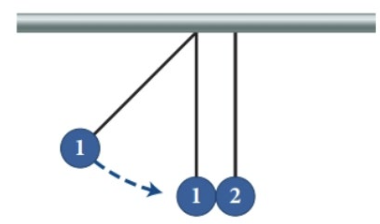
\includegraphics[width=0.5\linewidth]{../figures/E2122_1.png}
  \label{fig:E2122_1}
\end{figure}

To metalkugler, ophængt i tynde tråde fra en vandret stang, er til at begynde med i kontakt med hinanden, se \textbf{\autoref{fig:E2122_1}}. Kugle 1 har massen $m_1 = \qty{0,05}{kg}$, medens kugle 2 har massen $m_2 = \qty{0,10}{kg}$. Nu trækkes  $m_1$ (kugle 1) mod venstre, som vist i \textbf{\autoref{fig:E2122_1}}, og frigives, hvorefter den støder rent elastisk  sammen  med  $m_2$  (kugle  2).  I  øjeblikket  umiddelbart  før  stødet,  har  $m_1$  den  kinetiske  energi $K_1 = \qty{0,098}{J}$.

\subsection*{(a)}
Hvad er hastigheden af $m_1$ umiddelbart før stødet?
\bigbreak
Formlen for kinetisk energi $K$ er
\[ 
K = \frac{1}{2}mv^2
.\]
Hvor $m = \qty{0,05}{kg}$ er massen og $v$ er hastigheden. Heri kan hastigheden $v$ isoleres og kendte størrelser kan derefter indsættes som
\begin{align*}
  v_1 &= \sqrt{\frac{2K}{m}} \\
  &= \sqrt{\frac{2\cdot \qty{0,098}{J}}{\qty{0,05}{kg}}} \\
  &= \qty{1,98}{\frac{m}{s}} \approx \qty{2}{\frac{m}{s}} 
.\end{align*}
Altså har bolden med massen $m_1$ en hastighed $v_{1} = \qty{2}{\frac{m}{s}}$ umiddelbart før stødet.


\subsection*{(b)}
Bestem hastigheden af $m_1$ og hastigheden af $m_2$ umiddelbart efter stødet.
\bigbreak
Idet der er impulskonservation under stødet har vi at
\[ 
m_{1}\cdot v_{1i} + m_2 \cdot v_{2i} = m_1 \cdot v_{1f} + m_2 \cdot v_{2f} \implies m_1 v_{1i} + 0 = m_1 v_{1f} + m_2 v_{2f}
.\]
Restitutionskoefficienten for et komplet elastisk stød er $e = 1$ og er givet ved
\[ 
e = - \frac{v_{2f} - v_{1f}}{v_{2i} - v_{1i}} = 1 \implies v_{2f} - v_{1f} = v_{1i} \implies v_{2f} = v_{1i} + v_{1f}
.\]
Dette kan indsættes i udtrykket for impulskonservation som
\[ 
m_1 v_{1i} = m_1 v_{1f} + m_{2} (v_{1i} + v_{1f})
.\]
Heri kan $v_{1f}$ isoleres som
\begin{align*}
  m_2 v_{1i} + v_{1f} (m_1 + m_2) &= m_1 v_{1i} \\
  v_{1f} &= \frac{(m_1 - m_2) v_{1i}}{m_1 + m_2} \\
  &= \frac{\qty{0,05}{kg} - \qty{0,10}{kg}}{\qty{0,05}{kg} + \qty{0,10}{kg}}\cdot \qty{1,98}{\frac{m}{s}}  \\
  &= - \qty{0,66}{\frac{m}{s}} 
.\end{align*}

Idet hastigheden $v_{1f}$ nu er kendt kan formlen $v_{2f} = v_{1i} + v_{1f}$ nu benyttes som
\[ 
v_{2f} = \qty{1,98}{\frac{m}{s}} - \qty{0,66}{\frac{m}{s}} =  \qty{1,32}{\frac{m}{s}} 
.\]
Altså er hastighederne af $m_1$ og $m_2$ umiddelbart efter stødet hhv. $v_{1f} = - \qty{0,66}{m \per s}$ og $v_{2f} = \qty{1,32}{m \per s}$.


\subsection*{(c)}
Bestem restitutionskoefficienten $e$ for stødet.
\bigbreak
Idet stødet er komplet elastisk er restitutionskoefficienten, per definition, $e = 1$. Dette bekræftes imidlertid også ved brug af formlen idet
\[ 
  e = - \frac{\qty{1,32}{\frac{m}{s}} + \qty{0,66}{\frac{m}{s}}}{0 - \qty{1,98}{\frac{m}{s}}} = 1
.\]


\subsection*{(d)}
Forsøget gentages nu med to lerkugler. Det antages, at stødet er rent plastisk (rent uealstisk), således at de to kugler hænger sammen efter stødet. Bestem hastigheden af $m_1$ og $m_2$ umiddelbart efter stødet for dette tilfælde.
\bigbreak
For et komplet inelastisk stød sidder de to objekter sammen til sidst og de får derfor en fælleshastighed $\Vec{v}_2$. Impulskonservation giver os da at
\[ 
m_1 \cdot \Vec{v}_{1i} + m_2 \Vec{v}_{2i} = (m_1 + m_2)\Vec{v}_{2}
.\]
Idet $\Vec{v}_{2i} = 0$ kan $\Vec{v}_2$ isoleres og findes som
\begin{align*}
  \Vec{v}_2 &= \frac{m_1 \cdot \Vec{v}_{1i}}{m_1 + m_2} \\
  &= \frac{\qty{0,05}{kg} \cdot \qty{1,98}{\frac{m}{s}}}{\qty{0,05}{kg} + \qty{0,10}{kg}} \\
  &= \qty{0,66}{\frac{m}{s}}  \\
.\end{align*}
Altså vil de to lerkugler efter det komplet inealstiske sammenstød have en fælleshastighed $\Vec{v}_2 = \qty{0,66}{m\per s}$


\subsection*{(e)}
Bestem restitutionskoefficienten $e$ for det plastiske/uelastiske stød.
\bigbreak
For et komplet uelastisk stød er restitutionskoefficienten $e = 0$, per definition. Igen bekræftes dette af formlen for restitutionskoefficienten idet denne, idet de to objekter har samme hastighed efter stødet, får en tæller på 0 og dermed en samlet størrelse på 0. 


\section*{3.}
Et ``puf'' af komprimeret luft (trykluft) skubber et hagl ud af løbet af en luftpistol. Kraften, hvormed trykluften påvirker haglet, er givet ved $F(t) = F_0 e^{-\frac{t}{\tau}}$, hvor $t$ er tiden ($t \geq 0$), og $\tau$ (også med enheden tid) kaldes for en tidskonstant. (Der gælder også at $\tau > 0$).

\subsection*{(a)}
Hvad repræsenterer konstanten $F_0$?
\bigbreak
$F_0$ angiver størrelsen på $F(t)$ til tiden $t = 0$. Dette kan bekræftes ved at sætte $t = 0$ i eksponenten til $e$ hvorved eksponenten bliver 0 og højresiden af formlen derfor blot bliver $F_0$. 

\subsection*{(b)}
Skuddet (haglet) affyres til tiden $t = 0$. Hvad er haglets bevægelsesmængde (el. impuls) til tiden $t = \tau$?
\bigbreak
Det gælder generelt at impulsen kan findes som
\[ 
P = \int_{t_1}^{t_2} F(t) \, \mathrm{d}t
.\]
Dette integral kan løses som
\begin{align*}
  P &= F_0 \int_{0}^{\tau} e^{-\frac{t}{\tau}} \, \mathrm{d}t  \\
  &= F_0 \left[ -\tau e^{-\frac{t}{\tau}} \right]_{0}^{\tau}\\
  &= F_0 \cdot \left( \left( -\tau \cdot e^{-1} \right) - \left( -\tau \right) \right) \\
  &= F_0 \left( \tau - \tau e^{-1} \right) \\
  &= F_0 \tau \left( 1 - e^{-1} \right)
.\end{align*}


\subsection*{(c)}
Hvad er haglets bevægelsesmængde til tiden $t = 5\tau$?
\bigbreak
Her kan samme integral som før benyttes, dog med en ny øvre integrationsgrænse på $t = 5\tau$. Altså fås
\begin{align*}
  P &= F_0 \int_{0}^{5\tau} e^{-\frac{t}{\tau}} \, \mathrm{d}t  \\
  &= F_0 \left[ -\tau e^{-\frac{t}{\tau}} \right]_{0}^{5\tau} \\
  &= F_0 \cdot \left( \tau -\tau \cdot e^{-5} \right)  \\
  &= F_0 \tau (1-e^{-5})
.\end{align*}



\subsection*{(d)}
Hvad er haglets bevægelsesmængde efter meget lang tid ($t \to \infty$).
\bigbreak
Her kan samme integral som før igen benyttes men med en ny øvre integrationsgrænse på $\infty$. Altså fås, at
\begin{align*}
  P &= F_0 \int_{0}^{\infty} e^{-\frac{t}{\tau}} \, \mathrm{d}t  \\
  &= F_{0}\tau \left( 1 - e^{-\infty } \right) \\
  &= F_0 \tau \cdot (1-0) \\
  &= F_0 \tau
.\end{align*}


\subsection*{(e)}
Lad $\tau$ være lig med \qty{0,5}{ms} (\unit{ms} = milisekunder). Bestem tiden $t$, hvor haglets bevægelsesmængde har nået 95\% af sin slutværdi.
\bigbreak
Eftersom $\tau = \qty{0,5}{ms} \ll \infty$ har vi at $P_{max} = F_0 \cdot \qty{0,5}{ms} $. Dermed ønskes, at finde ud af, til hvilken tid $P = \num{0,95} F_0 \tau \cdot \qty{0,5}{ms} = F_0 \cdot \qty{0,475}{ms}$. Vi kan benytte integralet fra før men denne gang med en variabel integrationsgrænse $t$ som
\begin{align*}
  P(t) &= F_0 \int_{0}^{t} e^{-\frac{t}{\qty{0,5}{ms}}} \, \mathrm{d}t \\
  &= F_0 \cdot \left[ -\qty{0,5}{ms} \cdot e^{-\frac{t}{\qty{0,5}{ms}}} \right]_0^{t} \\
  &= F_0 \cdot \qty{0,5}{ms} \cdot  \left( 1 - e^{-\frac{t}{\qty{0,5}{ms}}} \right)
.\end{align*}
Dette udtryk for bevægelsesmængden som funktion af tiden $P(t)$ kan nu sættes lig den ønskede bevægelsesmængde $P = F_0 \cdot \qty{0,475}{ms}$ som
\begin{align*}
  F_0 \cdot \qty{0,475}{ms} &= F_0 \cdot \qty{0,5}{ms} \cdot \left( 1-e^{-\frac{t}{\qty{0,5}{ms}}} \right) \\
  \frac{\qty{0,475}{ms} }{\qty{0,5}{ms}} &= 1 - e^{-\frac{t}{\qty{0,5}{ms}}} \\
  e^{-\frac{t}{\qty{0,5}{ms}}} &= 1- \num{0,95} \\ 
  -\frac{t}{\qty{0,5}{ms}} &= \ln \num{0,05} \\
  t &= - \ln \num{0,05} \cdot \qty{0,5}{ms}  \\
  t &= \qty{1,498}{ms} \approx \qty{1,5}{ms}  \\
.\end{align*}


\section*{4.}
\begin{figure} [ht]
  \centering
  \caption{}
  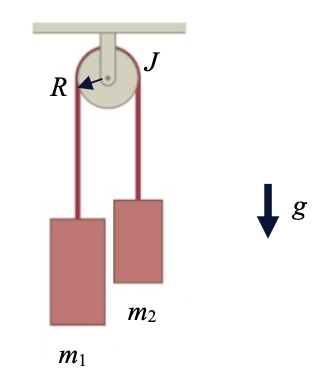
\includegraphics[width=0.5\linewidth]{../figures/E2122_2.png}
  \label{fig:E2122_2}
\end{figure}

En snor er lagt omkring en trisse med radius $R = \qty{0,30}{m}$ og masseinertimoment $J = \qty{0,80}{kg.m^2}$, se \textbf{\autoref{fig:E2122_2}}. I snorens ene ende er påsat massen $m_1 = \qty{3,0}{kg}$, i snorens anden ende massen $m_2 = \qty{2,0}{kg}$. Der kan ses bort fra snorens masse. Ligeledes kan det antages, at snoren ikke glider omkring trissen, og at snoren er ustrækkelig. De to masser understøttes først, for derefter at blive frigivet, til tiden $t = 0$. Tyngdeaccelerationen $g$ kan antages at være $g = \qty{9,80}{m\per s^2}$.

\subsection*{(a)}
Bestem accelerationen af hver af de to masser.
\bigbreak
Vi kan opskrive en kraftligevægt for begge de to masser som
\begin{equation} \label{eq:1}
  \sum F_t = 0; \qquad m_1\cdot g + (-m_1 a) -  T_1 = 0 \quad \implies \quad T_1 = m_1( g-a)
\end{equation}
og
\begin{equation} \label{eq:2}
  \sum F_t = 0; \qquad  - m_2g + (-m_2 a) + T_2 = 0 \quad \implies \quad - T_2 = -m_2 (a+g)
\end{equation}
Derudover har vi fra Newtons 2. lov for et roterende rigidt legeme at
\begin{equation} \label{eq:3}
  I \alpha = (T_1 - T_2) R
\end{equation}
Derudover har vi at den tangtielle acceleration for trissen, må tilsvare accelerationen af snoren, idet der ikke er et glid mellem de to. Altså
\begin{equation} \label{eq:4}
  a = \alpha R \implies \alpha = \frac{a}{R}
\end{equation}
Sættes \textbf{\autoref{eq:4}} ind i \textbf{\autoref{eq:3}} fås at
\[ 
I \frac{a}{R} = (T_1 - T_2) R \implies T_1 - T_2 = I \frac{a}{R^2}
.\]
Dermed har vi at
\begin{align*}
  m_1 (g-a) - m_2 (a+g) &= I \frac{a}{R^2} \\
  m_1g - m_1a - m_2a - m_2g &= I \frac{a}{R^2} \\
  I \frac{a}{R^2} + m_1 a + m_2 a &= m_1 g - m_2g \\
  a(\frac{I}{R^2} + m_1 + m_2) &= g(m_1 - m_2) \\
  a &= \frac{m_1 - m_2}{\frac{I}{R^2} + m_1 + m_2}g \\
  &= \frac{\qty{3,0}{kg} - \qty{2,0}{kg}}{\frac{\qty{0,80}{kg.m^2}}{\left( \qty{0,30}{m}  \right)^2} + \qty{3,0}{kg} + \qty{2,0}{kg}} \cdot \qty{9,80}{\frac{m}{s^2}}  \\
  &= \qty{0,706}{\frac{m}{s^2}} 
.\end{align*}


\subsection*{(b)}
Bestem trissens vinkelhastighed $\omega$ til det tidspunkt, hvor den tungeste masse $m_1$ har bevæget sig distancen $s = \qty{1,5}{m}$ nedad.
\bigbreak
Idet kræfterne alle er konstante, må det gælde at accelerationen fundet ovenfor ligeledes er konstant. Altså skal vi blot finde tidspunktet til $s = \qty{1,5}{m}$. Dette gøres med formlen for strækning ved konstant acceleration på kassen med $a = \qty{0,706}{\frac{m}{s^2}}$. Dette gøres som
\begin{align*}
  x &= x_0 + v_{0x}t + \frac{1}{2}at^2 \\
  x &= \frac{1}{2}at^2 \\
  t &= \sqrt{\frac{2x}{a}} \\
  t &= \sqrt{\frac{2 \cdot \qty{1,5}{m} }{\qty{0,706}{\frac{m}{s^2}}}} \\
  t &= \qty{2,06}{s}
.\end{align*}
Vi kan beregne trissens vinkelacceleration $\alpha$ som
\[ 
\alpha = \frac{a}{R} = \frac{\qty{0,706}{\frac{m}{s^2}}}{\qty{0,30}{m}} = \qty{2,35}{s^{-2}} 
.\]
Idet det antages at trissen ikke har nogen hastighed inden de to masser bliver frigivet må det gælde at vinkelhastigheden $\omega$ til tiden $t$ kan findes som
\[ 
  \omega = \alpha t = \qty{2,35}{s^{-2}} \cdot \qty{2,06}{s}  = \qty{4,84}{s^{-1}} 
.\]


\subsection*{(c)}
Bestem snorkræfterne (i begge ender af snoren), til samme tidspunkt.
\bigbreak
Snorkræften er konstant, for den gældende bevægelse, så snorkraften til $t = \qty{1,5}{s}$ er lig snorkraften til alle andre tidspunkter. Vi har allerede fundet et udtryk for snorkraften over $m_1$; $T_1$ og for snorkraften over $m_2$; $T_2$ og vi sætter derfor bare kendte størrelser ind i denne som
\begin{align*}
  T_1 &= m_1 (g - a) = \qty{3,0}{kg} \left( \qty{9,80}{\frac{m}{s^2}} - \qty{0,706}{\frac{m}{s^2}}  \right) = \qty{27,3}{N} \\ 
  T_2 &= m_2 (a + g) = \qty{2,0}{kg} \left( \qty{9,80}{\frac{m}{s^2}} + \qty{0,706}{\frac{m}{s^2}}  \right) = \qty{21,0}{N} 
.\end{align*}


\subsection*{(d)}
Bestem den øjeblikkelige effekt som de to masser tilfører trissen via snoren, til samme tidspunkt.
\bigbreak
Vi har at effekten $P$ kan findes som
\[ 
P = \omega \tau = (T_1 - T_2)R\omega
.\]
Sættes kendte størrelser ind fås at
\[ 
P = \left( \qty{27,3}{N}  - \qty{21,0}{N}  \right) \cdot \qty{0,30}{m} \cdot \qty{4,84}{s^{-1}} = \qty{9,15}{W} 
.\]


\end{document}
